% ........................................................................... %

This chapter presents the model of \emph{timed business protocols}. It is a formalization of the business protocol introduced in \cite{FTBB} and the timing constraints primitives that were mentioned in \cite{BBFC04,BCT-CAISE03}. By investigating (online) applications to define which type of timing abstraction would turn out to be useful in practice for describing the externally-observable behavior of services, we identified two primitives: \CInvoke constraints for defining time windows of availabilities and \MInvoke constraints for defining implicit actions that occur when some forms of delays expire. The introduction of timing constraints into the model poses significant challenges, especially when it comes to studying the impacts on protocol analysis as we will see in the next chapters. We obtained a characterization of timed protocols and their operators by establishing a link with the field of timed automata \cite{RADLD94}. This way, we will see that introducing timing constraints in business protocols is a significant challenge as it makes protocol analysis much more complex than in the untimed case. More specifically, we will see that with timed automata, complementation and subsumption are generally undecidable while \MInvoke constraints are hard to express. \\

The chapter is structured as follows. We first provide a concise discussion on the timing abstractions that we identified. Then, we present the model of timed business protocols that we envisioned as a conceptual model. Next, we explain how timed protocols can be equivalently expressed using \emph{timed automata} \cite{RADLD94}, a formal framework that has been extensively investigated in formal verification research works \cite{RAPM04,UPPAAL}. This will later allow us to derive theoretical properties for the model of timed protocols by establishing a semantic-preserving mapping between the two models. Finally, we provide a discussion.

% ........................................................................... %

\section{Timing abstractions}

% ........................................................................... %

Before designing our web services business protocols model, we started by investigating the timing abstractions that were needed to capture the ones that would be useful in practice. We first present three motivating examples, then introduce the two timing abstraction primitives that we have identified.

% ........................................................................... %

\subsection{Motivating examples}

Timing constraints appear in countless scenarios. We give here three examples related to web services and business processes were timing constraints play a critical role.

% ........................................................................... %

\subsubsection{E-Commerce portals}

The sales conditions notices of many E-Commerce portals provide timing constraints. Let us consider a classic example of a plane ticket seller portal. A potential purchaser is usually allowed to put a seat on hold for a day or two before a confirmation involving the effective payment is made. The seller implicitly releases the seat holding and cancels the purchase process after a delay (e.g., 24 hours) without a confirmation or canceling notification from the buyer. There are other examples in the field of E-Commerce examples. For example goods selling portals are usually entitled by law regulations to allow a buyer to return a purchase within a short delay such as one week after the delivery. They are often also constrained to respect delays when dealing with customers for operations such as the deliveries or the refunding of returned purchases.

\begin{figure}[htbp]
    \centering
    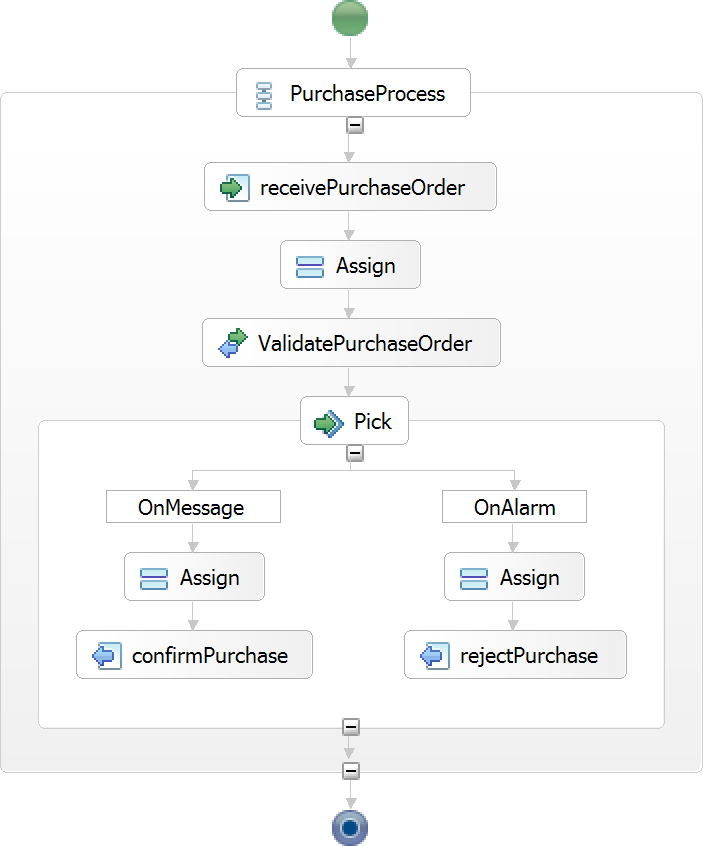
\includegraphics[height=11cm]{content/protocol-model/bpel-purchase}
    \caption{A BPEL process that uses an alarm.}
    \label{fig:bpel-purchase}
\end{figure}

\subsubsection{BPEL processes}

The \emph{Business Process Execution Language} \cite{WSBPEL2} is the major specification in the field of long-running web services orchestrations. A BPEL process is able to achieve a complex business process using a set of web services. Figure~\ref{fig:bpel-purchase} exhibits a sample purchasing BPEL process. The process starts by receiving a purchase order. A BPEL \emph{Assign} operation is then executed to prepare the data for the invocation of a service providing a \emph{ValidatePurchaseOrder} operation. This operation is used to delegate the processing of the purchase order to a service that will check for various conditions like the ordered items availability, the existence of contracts between the requesting entity and the provider, the validity of the chosen payment option and checking that the requesting entity does not have outstanding debts to the provider. Given that those checkings may take a substantial amount of time (for examples humans have to be involved for some of the checkings), the process uses a \emph{pick} block. It allows to wait for receiving a response that validates the order. If no response has been received after an arbitrary delay such as 48 hours, the process is woken-up to reject the purchase. BPEL actually exhibits two similar time-related constructs: \emph{onAlarm} and \emph{wait}. The former can be used in \emph{pick} blocks, while the later is a normal BPEL operation that will put the process execution on hold for a duration or until a fixed date is reached.

\begin{figure}[htbp]
    \centering
    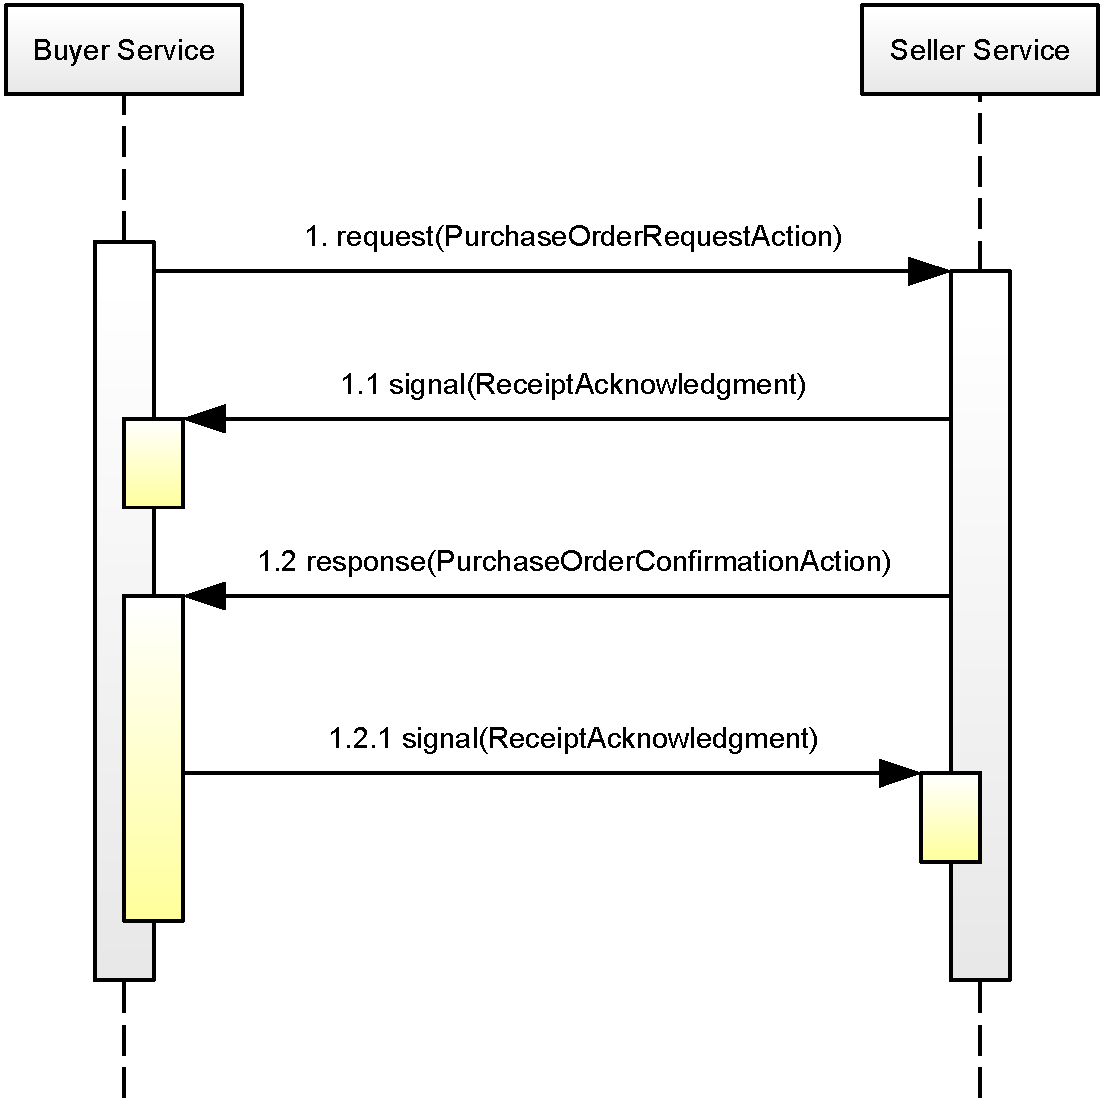
\includegraphics[width=\textwidth]{content/protocol-model/pip3a4}
    \caption{Sequence diagram of the RosettaNet PIP 3A4 (Request Purchase Order).}
    \label{fig:pip3a4}
\end{figure}

\subsubsection{RosettaNet PIPs}

RosettaNet \cite{ROSETTANET} is an industrial consortium which aims at facilitating the transactions among the supply chains of trading partners using specifications called the \emph{Partner Interface Processes} (PIPs) that thoroughly detail the processes involved in those transactions. The RosettaNet PIPs exhibit time-dependent behaviors. Let us focus on the PIP 3A4 depicted on Figure~\ref{fig:pip3a4}. It specifies how a seller and a buyer can process a purchase order. This PIP specifies the following timing constraints:
\begin{itemize}

    \item the \emph{PurchaseOrderRequestAction} and the \emph{PurchaseOrderConfirmationAction} must be acknowledged within 2 hours

    \item the reply to the \emph{PurchaseOrderRequestAction} must be sent within 24 hours.

\end{itemize}

% ........................................................................... %

\subsection{Timing abstraction primitives}

% ........................................................................... %

The three motivating examples that we gave illustrate the need for capturing timing abstractions into web services and business process models. We did not limit our investigations to these examples in order to identify the primitives that would be useful to capture the vast majority of cases appearing in practice. A major difficulty when designing a model is to find a good expressiveness level tradeoff. Indeed, a simplistic model does not capture all of the cases while an overly complex one becomes hard to use for practitioners, and may lead to undecidability problems in algorithms.\\

The starting point of this work was done in \cite{BCT-CAISE03,KBBB+04}. Using a similar approach based on the exploration of existing web portals and E-Commerce websites, we found that the following timing primitives would be useful.

\paragraph{Time windows.} Many actions need to be available only during certain time windows. For example, a quotation usually has a finite validity, and a purchase cannot be made in the same conditions once it has expired. Another example in the commerce domain is the case of discounts which can be valid only for a limited period of time.

\paragraph{Timeouts.} Most software systems support the notion of timeout, for example to avoid locking resources for an unlimited amount of time and to handle partnering components errors. Considering again an example in the commerce domain, a purchase order needs to be paid to be validated. A seller system will usually discard the business transaction after a given delay if the buyer did not actually send the payment.

% ........................................................................... %

\section{Extending business protocols with temporal abstractions}

% ........................................................................... %

We now present the \emph{timed business protocol} model. We first illustrate it informally, then provide a formalized definition.

% ........................................................................... %


\subsection{Timed business protocols}

% ........................................................................... %

Our model is an extension of the \emph{business protocol} model \cite{BBFC04,FTBB} which is built upon the traditional state-machine formalism. Indeed, it is commonly used to model the behavior of systems, due to the fact that it is simple and intuitive.
In the model, states represent the different phases that a service may go through during its interaction with a requester. A transition label is a message supported by the service. It has a polarity which is positive ($+$) if the message is incoming, or negative $(-)$ if it is outgoing. Transitions are triggered when their associated messages are sent or received. Hence, a state identifies a set of outgoing transitions, and therefore a set of possible messages that can be either sent or received when the conversation with a requester is in this state.\\

\begin{figure}[thbp]
    \centering
    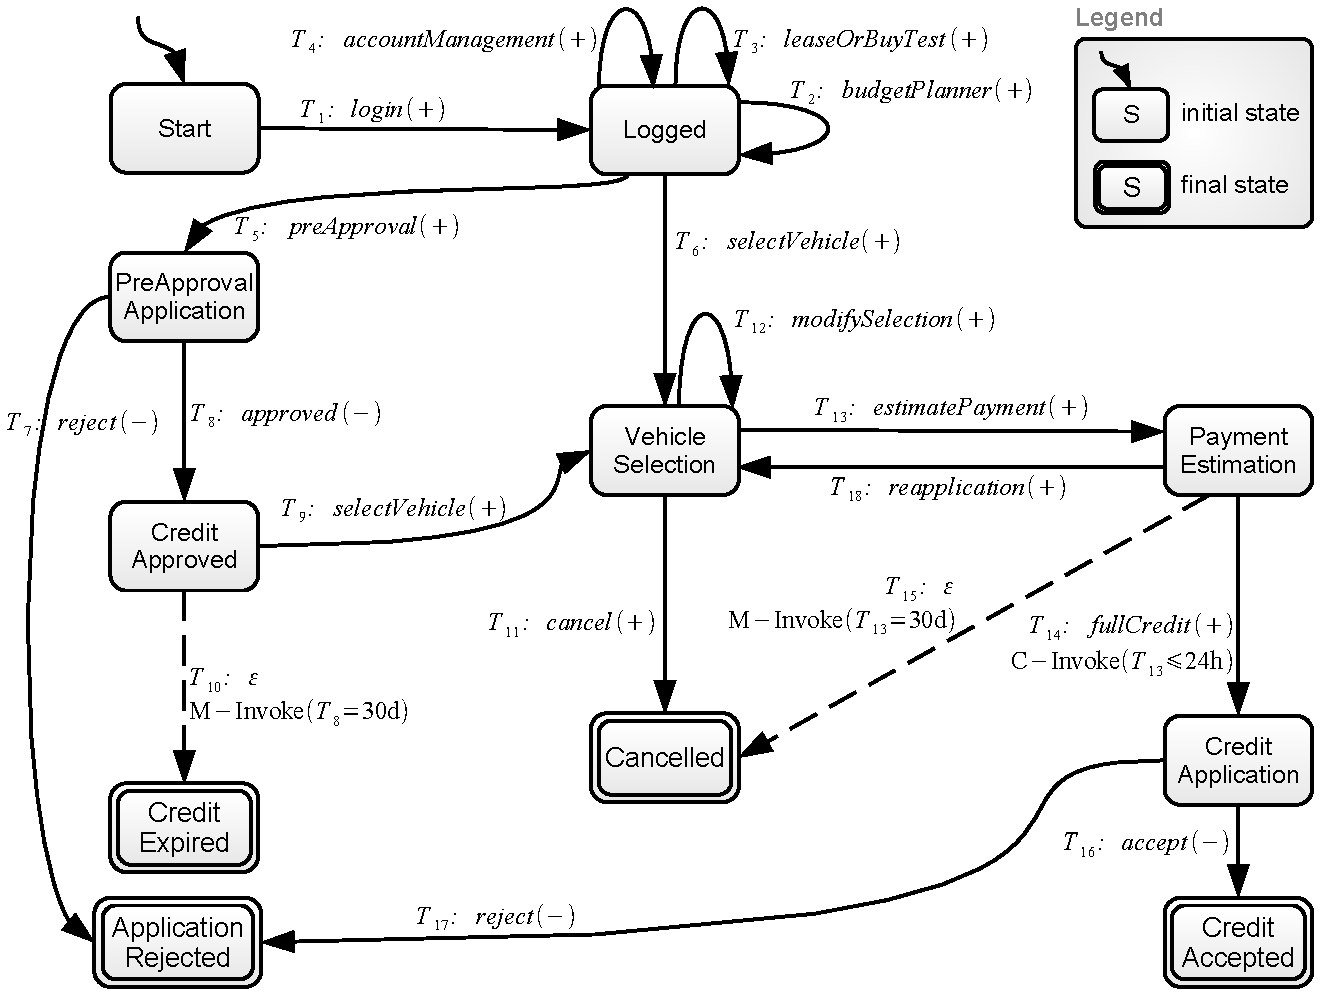
\includegraphics[width=\textwidth]{content/protocol-model/ford-credit}
    \caption{A timed protocol of an online financing service.}
    \label{fig:ford-credit}
\end{figure}

As an example, the protocol depicted on Figure~\ref{fig:ford-credit} (inspired by the \emph{Ford Credit web portal}) is initially in the $Start$ state, and requesters begin a conversation by sending a $login$ message, moving to the $Logged$ state.\\

In the figure, the initial state is indicated by an unlabeled entering arrow while final states are double-circled. A conversation is accepted when ending in such a final state. Hence, a sequence of messages $login(+) \cdot preApproval(+) \cdot reject(-)$ is a conversation supported by the protocol, while $selectVehicle(+) \cdot login(+)$ is not: no transition for a $selectVehicle$ message is available from the $Start$ state, the two messages cannot be ordered this way, and the conversation does not end in a final state.  Business protocols must be deterministic, as the requesters always need to be able to determine in which state the service is, else much of the purpose of the protocol specification would be lost.\\

We consider the following two extensions to the base protocol model:
\begin{enumerate}

    \item \CInvoke constraints specify time windows within which a transition \emph{can} be fired. Outside of those time windows, the transition is disabled, and exchanging the associated message results in an error.
    
    \item \MInvoke constraints specify \emph{when} a transition is \emph{automatically} fired.
    
\end{enumerate}

The obtained model  is called  \emph{timed (business) protocol model}.
\CInvoke constraints can be attached to \emph{explicit} transitions for which a message is exchanged between the service provider and its requesters. The absence of \CInvoke constraint on an explicit transition means that it can be fired from its source state at any time.
By contrast, \MInvoke constraints are associated to \emph{implicit} transitions. They model state changes in conversations once a delay has elapsed (a typical example being a timeout). They are not related to message exchanges between the service provider and its requesters. Implicit transitions are analogous to the silent transitions in the automata theory \cite{Hopcroft79} and we associate the empty word $\varepsilon$ as the label of those transitions. There is however a significant difference compared to ``classical'' automata: they cannot be removed in the general case as we will see later. \\

Continuing with the example protocol depicted on Figure~\ref{fig:ford-credit}, it is indicated that a full credit application is accepted only if it is received at most 24 hours after a payment estimation has been made. This behavior is specified by tagging the transition $T_{14}: fullCredit(+)$ with a time constraint $\CInvoke(T_{13} \leq 24h)$, i.e., $T_{14}$ can only be fired within a time window $[0h, 24h]$ after $T_{13}$ has been fired. $T_{10}$ has a constraint $\MInvoke(T_8 = 30d)$, meaning that once a pre-approval application has been approved ($T_8$), a requester is given 30 days to select a vehicle ($T_9$). If it does not continue the conversation by sending a $selectVehicle$ message within the next 30 days, then the service provider will automatically fire $T_{10}$ and move to the $CreditExpired$ state, ending the conversation. Finally, it should be noted that the presence of an implicit transition from a given state affects the time constraints of the explicit transitions outgoing from the same state. Indeed, $T_{10}$ implies that $T_9$ can only be fired within a time window matching the 30 days. Hence, a constraint $\CInvoke(T_8 < 30d)$ is implicitly associated with $T_9$ because of the \MInvoke constraint of $T_{10}$.\\

\begin{figure}[htbp]
    \centering
    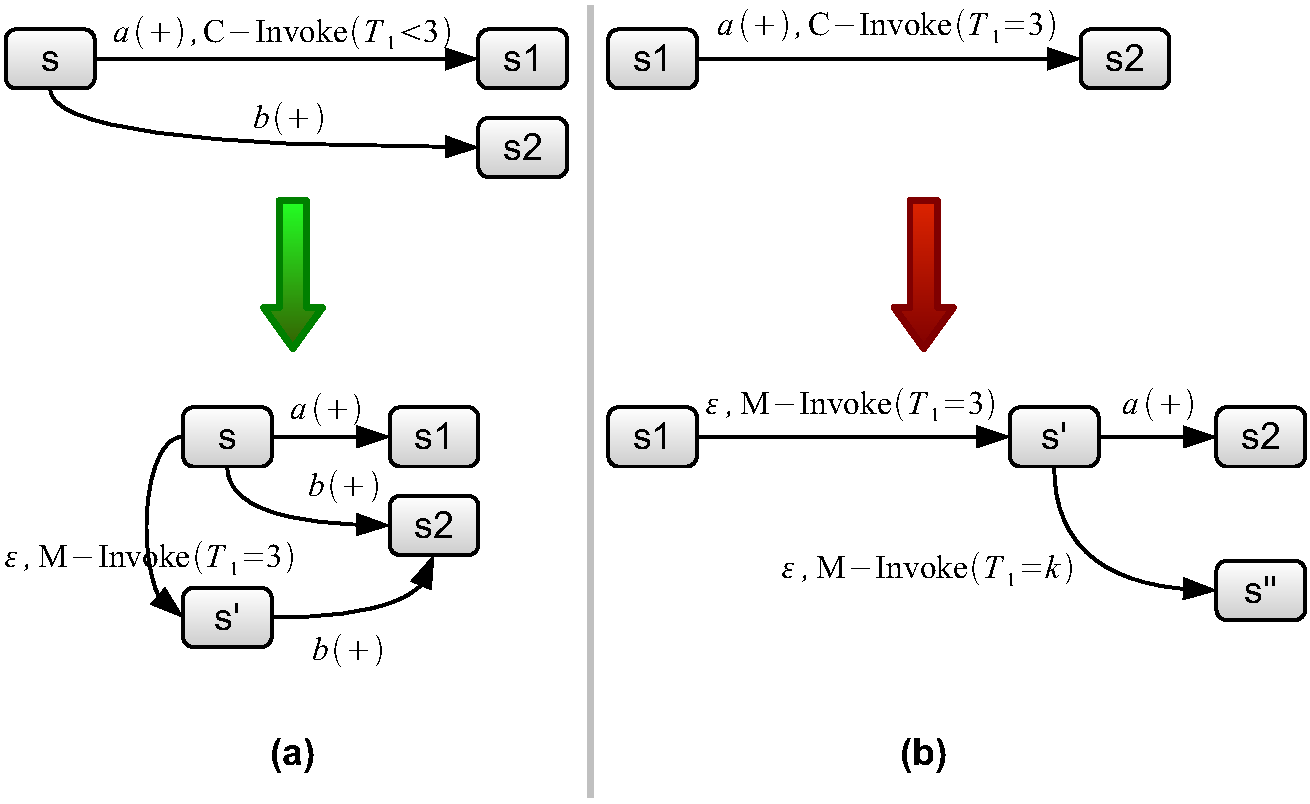
\includegraphics[width=\textwidth]{content/protocol-model/ci-vs-mi}
    \caption{Examples for illustrating why both \CInvoke and \MInvoke are necessary.}
    \label{fig:ci-vs-mi}
\end{figure}

Both \CInvoke and \MInvoke constraints are orthogonal. Indeed, we will see in Theorem~\ref{thm:mi-expressiveness} that the transitions having \MInvoke constraints strictly increase expressiveness of our model. Naturally, the usefulness of \CInvoke constraints can be questioned as in many cases, a \CInvoke-free construction can be made by using extra states and \MInvoke constraints on implicit transitions. Let us consider the examples of Figure~\ref{fig:ci-vs-mi}. The case (a) is simple as the \CInvoke constraint is easily translated using \MInvoke by adding an extra state $s'$.
This is however not true in the general case as the (b) counter example shows as it yields the following problem: $k \in \Q$ cannot be determined as the set of rational numbers is infinite, hence we cannot find a value for $k$ that would be ``close-enough'' to $3$ for ensuring that $a(+)$ is only received when $T_1$ is exactly equal to $3$.

% ........................................................................... %

\subsection{Formalization}

% ........................................................................... %

\subsubsection{Syntax}

% ........................................................................... %

Before giving the definition of timed protocols, we need to formalize the \CInvoke and \MInvoke constraints.
Let $\mathcal{X}$ be a set of variables referring to transition identifiers: if $r$ is a transition then $T_r \in {\mathcal{X}}$ is the variable referring to this transition. We consider the two kinds of time constraints defined over a set of variables $\mathcal{X}$ using the following grammars:
\begin{itemize}

    \item $\CInvoke{(c)}$ with  $c$ defined as follows:
    $$ c ::= x \; op \; k \; | \; x - x' \; op \; k \; | \; c \wedge c \; | \; c \vee c $$
    with  $op \in \{=, \neq, <, >, \leq, \geq\}$,
     $x \in \mathcal{X}$, $x' \in \mathcal{X}$ and $k \in \Q \cup \{ \perp \}$, where $\Q$ denotes the set of positive rational numbers,

    \item $\MInvoke{(c)}$ with $c$ defined as follows:
    $$ c ::= (x = k) \wedge c' \; | \; c \wedge c \; | \; c \vee c $$
    with $x \in \mathcal{X}$, $k \in \Q \cup \{ \perp \}$ and $c'$ being defined like in the grammar of \CInvoke constraints.

\end{itemize}

The following is the definition for timed business protocols, extending the business protocols model \cite{BBFC04,FTBB}.

\begin{definition}
A \emph{timed business protocol} is a tuple $\mathcal{P} = (\mathcal{S}, s_0, \mathcal{F}, \mathtt{M}, \mathcal{X}, \mathcal{C}, \mathcal{R})$ where:
\begin{itemize}

  \item $\mathcal{S}$ is a finite set of states, with $s_0 \in \mathcal{S}$ being the initial state.

  \item $\mathcal{F} \subseteq \mathcal{S}$ is the set of final states. If $\mathcal{F} = \emptyset$, then $\mathcal{P}$ is said to be an empty protocol.

  \item $\mathtt{M} = \mathtt{M_e} \cup \{\varepsilon\}$ is a finite set of messages $\mathtt{M_e}$ augmented with the empty message $\varepsilon$. For each message $m \in \mathtt{M_e}$, we define a function $\polarity{\mathcal{P}}{m}$ which will be positive $(+)$ if $m$ is an input message in $\mathcal{P}$, and negative $(-)$ if $m$ is an output message in $\mathcal{P}$.

  \item We assume that each transition $r \in \mathcal{R}$ is identified by a unique identifier $id(r)$. $\mathcal{X} = \{ T_i \;|\; \exists r \in \mathcal{R},\; T_i = id(r) \}$ is a set of clock variables defined over the set of transitions $\mathcal{R}$.

  \item $\mathcal{C}$ is a set of time constraints defined over a set of variables $\mathcal{X}$. The absence of a constraint is interpreted as a constraint which always evaluates to $\mathtt{true}$.

  \item $\mathcal{R} \subseteq \mathcal{S}^2 \times \mathtt{M} \times \mathcal{C}$ is a finite set of transitions.
  Each transition $(s, s', m, c)$ identifies a source state $s$, a target state $s'$, a message $m$ and a constraint $c$. We say that the message $m$ is enabled from a state $s$. When $m = \varepsilon$, $c$ must be a \MInvoke constraint,  otherwise $c$ must be either a \CInvoke constraint or $\mathtt{true}$.

\end{itemize}
\end{definition}

In the sequel, we use the notation $\mathcal{R}(s, s', m, c)$ to denote the fact that $(s, s', m, c) \in \mathcal{R}$. To enforce determinism, we require that a protocol has only one initial state, and  that for every state $s$ and every two transitions $(s, s_1, m_1, c_1)$ and $(s, s_2, m_2, c_2)$ enabled from $s$, we have either $m_1 \neq m_2$ or $c_1 \wedge c_2 \equiv \mathtt{false}$.

% ........................................................................... %

\subsubsection{Semantics}

% ........................................................................... %

\paragraph{Variable interpretation.}
Defining the timed protocol semantics requires the introduction of the notion of variable valuation. We consider as a time domain the set of positive reals $\Rpos$ augmented with a special element $\perp$ to denote the fact that a transition has never been taken yet.
Let $\mathcal{X}$ be a set of variables valued in $\Rpos$. A variable valuation
$$ \val : {\mathcal{X}} \rightarrow \Rpos \cup \{ \perp \} $$
is a mapping that assigns to each variable $x \in {\mathcal{X}}$ a time value $\val(x)$.\\

We note by $\val_{t}(x)$ the valuation of $x$ at an instant $t$. In the beginning (i.e., at instant $t_0 = 0$) we assume that all of the variables are set to $\perp$, i.e., $\val_{{t_0}}(T_i) = \perp, \forall T_i \in {\mathcal{X}}$.\\

Then, a variable valuation at a time $t_j$ is completely determined by a protocol execution. Consider for example an execution $\sigma = s_0 \cdot (m_0, t_0) \cdot s_1 \ldots s_{n-1}.(m_{n-1}, t_{n-1}) \cdot s_n$ of a protocol $\mathcal{P}$. The valuation of a clock variable $T_i$ at time $t_j$, with $0 < j \leq n$, is defined as follows:
$$
\val_{{t_j}}(T_i) =
\left \{
  \begin{array}{l}
  
    \val_{t_{j-1}}(T_i) + (t_j - t_{j-1}) \\
    
    0 \mbox{ if } T_i = id(\mathcal{R}(s_j, s_{j+1}, m, c)) \mbox{ is fired from  } s_j \mbox{ to } s_{j+1} \\
  
  \end{array}
\right.
$$
It should be noted that for any $r \in \Rpos$, $k \in \Q$ and any comparison operator $op \in \{<, \leq, =, \neq, >, \geq \}$:
$$
\left\lbrace
\begin{array}{l}
  \perp +\; r =\; \perp \\
  \perp -\; r =\; \perp \\
  \perp op\; k = \mathtt{false} \\
  \perp op \perp \; = \mathtt{true} \mbox{ if } op \in \{ =, \leq, \geq \} \\
  \perp op \perp \; = \mathtt{false} \mbox{ otherwise }\\
\end{array}
\right.
$$

Given a variable valuation $\val$ and a constraint $\CInvoke{(c)}$ (respectively, $\MInvoke{(c)}$), we note by $c(\val)$, the constraint obtained by substituting each variable $x$ in $c$ by its value $\val(x)$. A variable valuation $\val$ satisfies a constraint $\CInvoke{(c)}$ (respectively, $\MInvoke{(c)}$) if and only if
$c(\val) \equiv \mathtt{true}$. In this case, we write $\val\ \models \CInvoke{(c)}$ (respectively, $\val \models \MInvoke{(c)}$)

\paragraph{Timed conversations.}
Timed conversations are inspired from the notion of \emph{timed words} in timed automata as defined in \cite{RADLD94}.\\

Let $\mathcal{P} = (\mathcal{S}, s_0, \mathcal{F}, \mathtt{M}, \mathcal{X}, \mathcal{C}, \mathcal{R})$ be a timed protocol. A \emph{correct execution} (or simply, an execution) of $\mathcal{P}$ is a sequence $\sigma = s_0 \cdot (m_0, t_0) \cdot s_1 \ldots s_{n-1} \cdot (m_{n-1}, t_{n-1}) \cdot s_n$  such that:
\begin{enumerate}

    \item $t_0 \leq t_1 \leq \ldots \leq t_n$ (i.e., the occurrence of times increase monotonically),

    \item $s_0$ is the initial state and $s_n$ is a final state of $\mathcal{P}$, and

    \item $\forall j \in [1,n]$, we have: $\mathcal{R}(s_{j-1}, s_{j}, m_{j-1}, c_{j-1})$ and $\val_{j-1} \models c_{j-1}$.
\end{enumerate}

\begin{sloppypar}
As an example, the sequence
$\sigma' = Start \cdot (login(+), 0) \cdot Logged \cdot (preApproval(+), 1) \cdot PreApprovalApplication
\cdot (approved(-), 3) \cdot CreditApproved \cdot (\varepsilon, 33) \cdot CreditExpired$
is a correct execution of the financing service protocol depicted on Figure~\ref{fig:ford-credit}.
\end{sloppypar}\

If $\sigma = s_0 \cdot (m_0, t_0) \cdot s_1 \ldots s_{n-1} \cdot (m_{n-1}, t_{n-1}) \cdot s_n$ is a correct execution of $\mathcal{P}$, then the sequence $tr(\sigma) = (m_0, t_0) \ldots (m_{n-1}, t_{n-1})$ forms a \emph{timed trace} which is compliant with  $\mathcal{P}$.
Continuing with the example, the execution $\sigma'$ of the above service protocol leads to the timed trace $tr(\sigma') = (login(+), 0) \cdot (preApproval(+), 1) \cdot (approved(-), 3) \cdot (\varepsilon, 33)$.\\

During an execution $\sigma$ of a protocol $\mathcal{P}$, the externally observable behavior of $\mathcal{P}$, hereafter called \emph{timed conversation} of $\mathcal{P}$ and noted $conv(\sigma)$, is obtained by removing from the corresponding timed trace $tr(\sigma)$ all of the non observable events (i.e., all of the pairs $(m_i, t_i)$ with $m_i = \varepsilon$). For example, during the previous execution $\sigma'$, the observable behavior of the financing service is described by the timed conversation $obs(\sigma') = (login(+), 0) \cdot (preApproval(+), 1) \cdot (approved(-), 3)$.\\

In the following, given a protocol $\mathcal{P}$, we denote by $Tr(\mathcal{P})$  the set of timed conversations of $\mathcal{P}$.

\paragraph{Timed interactions.}
Timed conversations describe the externally observable behavior of timed protocols and, as we will show below, are essential to analyze the ability of two services to interact correctly.
Consider for example the protocol $\mathcal{P}$ depicted on Figure~\ref{fig:ford-credit} and its reversed protocol $\mathcal{P'}$ obtained by reversing the polarity of the messages (i.e., input messages become outputs and vice-versa).

\begin{sloppypar}
We can observe that when $\mathcal{P'}$  interacts with $\mathcal{P}$ by following a given timed conversation, $\mathcal{P}$ follows exactly a conversation with the reversed polarities of the messages. For example, if during such an interaction the timed conversation of $\mathcal{P}$ is $(login(+), 0) \cdot (selectVehicle(+), 1) \cdot (estimatePayment(+), 10) \cdot (fullCredit(+), 30) \cdot (accept(-), 100)$, then the timed conversation of $\mathcal{P'}$ is $(login(-), 0) \cdot (selectVehicle(-), 1) \cdot (estimate\-Payment(-), 10) \cdot (fullCredit(-), 30) \cdot (accept(+), 100)$.
\end{sloppypar}\

\begin{sloppypar}
In this case, we call the path $(login, 0) \cdot (selectVehicle, 1) \cdot (estimatePayment, 10) \cdot (fullCredit, 30) \cdot (accept, 100)$ a \emph{timed interaction trace} of $\mathcal{P}$ and $\mathcal{P'}$. The polarities of the messages that appear in interaction traces are not defined. Indeed, each input message $m$ of one protocol matches an output message $m$ of the other protocol.
\end{sloppypar}\

More precisely, let $\mathcal{P}$ and $\mathcal{P}'$ be two timed protocols and let $\tau = (a_0, t_0) \cdot (\ldots) \cdot (a_n, t_n)$ be a sequence of events in which the polarities of the messages are undefined. Then $\tau$ is a timed interaction trace of $\mathcal{P}$ and $\mathcal{P}'$ if and only if there exist two timed conversations $\sigma_1$ and $\sigma_2$ such that:
\begin{enumerate}

    \item $\sigma_1 \in Tr(\mathcal{P})$ and  $\sigma_2 \in Tr(\mathcal{P}')$, and

    \item $\sigma_1$ is the reverse conversation of $\sigma_2$ (i.e., the conversation obtained from $\sigma_2$ by inverting the polarities of the messages), and

    \item $\tau = Unp(\sigma_1) = Unp(\sigma_2)$ where $Unp(\sigma)$ denotes the trace obtained from $\sigma$ by removing the polarities of the messages.

\end{enumerate}

% ........................................................................... %

\section{From timed protocols to protocol timed automata}

% ........................................................................... %

The previous section has introduced the model of timed business protocols which is suitable for describing the external behavior of web services, including timing constraints. In turn, the model of timed automata \cite{RADLD94} has been extensively studied as an extension of classical automata \cite{Hopcroft79} with real-valued clocks and conditions on the transitions. Given the extensive research that has been made on timed automata, we chose to:
\begin{enumerate}
  
  \item use timed protocols as a conceptual model, and
  
  \item use timed automata for implementing the behavior of timed protocols, and
  
  \item derive theoretical properties of timed protocols from existing work on timed automata.
  
\end{enumerate}
To do that, we give a mapping from timed protocols to a new class of timed automata that we identified, called \emph{protocol timed automata}. However, defining such a mapping is not a trivial task as we will see that \MInvoke constraints are not straightforward to implement using timed automata.\\  

This section is structured as follows. We start by an informal, illustrated walk through the challenges of converting a timed protocol to a timed automaton that correctly implements its behavior. We then briefly define the class of protocol timed automata. Then, we formally study the \MInvoke constraints enforcement techniques for timed automata.

% ........................................................................... %

\subsection{Informal overview of the challenges}

% ........................................................................... %

\begin{figure}[htbp]
    \centering
    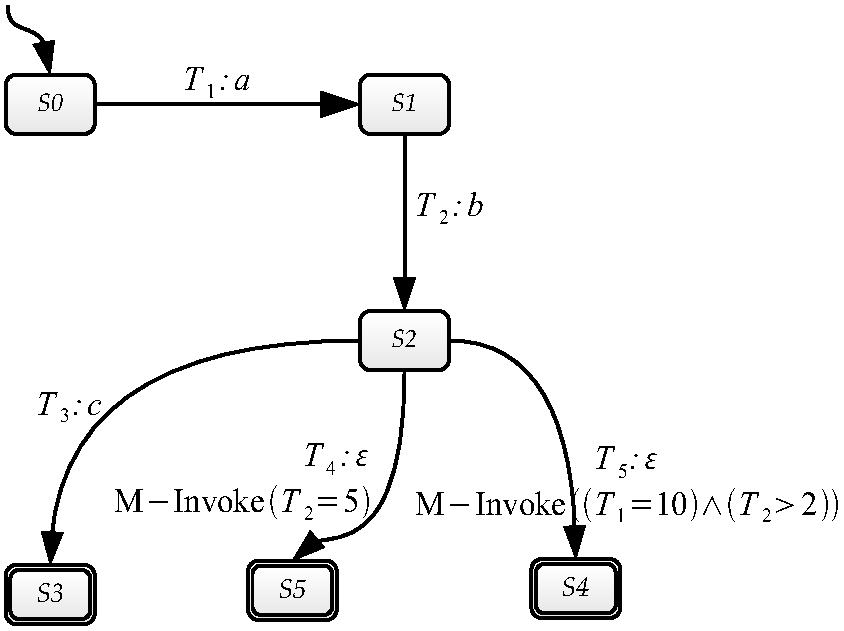
\includegraphics[width=\textwidth]{content/protocol-model/pta-protocol}
    \caption{A sample timed protocol $\mathcal{P}$ used as a mapping running example.}
    \label{fig:pta-protocol}
\end{figure}

We will use the timed protocol from Figure~\ref{fig:pta-protocol} as a running example throughout this section. It will allow us to illustrate the challenges in creating a timed automaton that behaves like a timed protocol. At first sight, the translation may look straightforward. However as we will see, preserving the behavior of \MInvoke is surprisingly not an easy task. The translation is performed using a mapping that we now illustrate. The mapping is done in two steps.\\

The first step to convert a timed protocol $\mathcal{P}$ into a timed automaton $A$ is relatively simple. The mapping of the states of $\mathcal{P}$ to the locations of $A$ is direct (e.g., the state $s_0$ of $\mathcal{P}$ is mapped to a location $l_0$). Similarly, each transition in $\mathcal{P}$ is translated as a switch with the message name as its label (e.g., in $\mathcal{P}$, $T_1: \mathcal{R}(s_0, s_1, a, \mathtt{true})$ is translated as a switch $e_1 = (l_0, \mathtt{true}, a, r, l_1)$ in $A$). Also, the initial location and the final locations in $A$ correspond to the initial and final states in $\mathcal{P}$.\\

\begin{figure}[htbp]
    \centering
    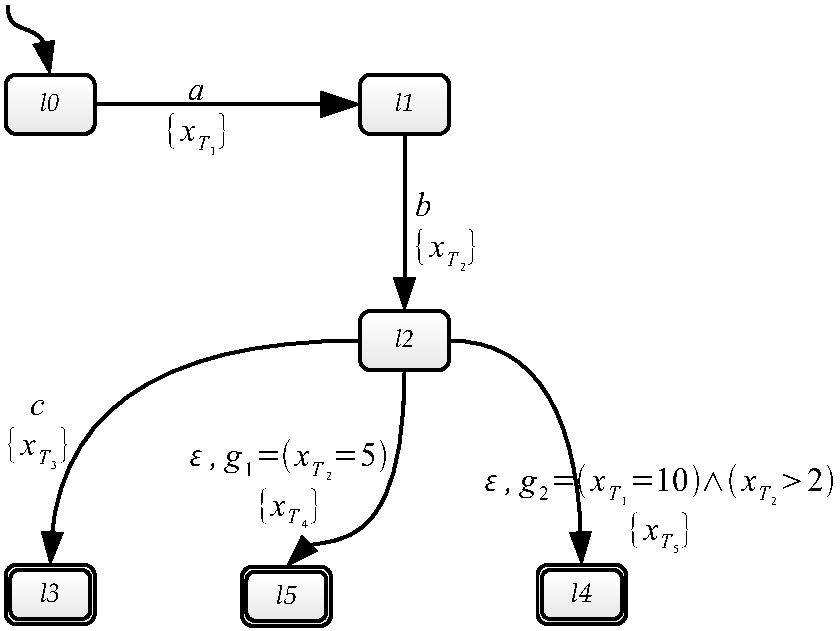
\includegraphics[width=\textwidth]{content/protocol-model/bogus-pta-constraint}
    \caption{A sample timed automaton that does not enforce M-Invoke semantics.}
    \label{fig:bogus-pta-constraint}
\end{figure}

The transition identifiers from $\mathcal{P}$ are used to generate clocks in $A$. Indeed, each identifier generates a unique clock which is solely reset on its corresponding switch. For example the transition $T_2$ generates a clock $x_{T_2}$ in $A$ which is only reset on the switch that was mapped from $T_2$. This way, we can know when a switch was fired, just like in the timed protocol $\mathcal{P}$. The conversion of a \CInvoke constraint from $\mathcal{P}$ is also direct. For example, a constraint $\CInvoke(T_1 < 3)$ is mapped to a guard $(x_{T_1} < 3)$. At this stage, the mapping of $\mathcal{P}$ to $A$ yields the timed automaton of Figure~\ref{fig:bogus-pta-constraint}.\\

Assuming that we mapped implicit transitions as $\varepsilon$-labeled switches with a direct translation of \MInvoke constraints into guards, the following problems arise on the timed automaton of Figure~\ref{fig:bogus-pta-constraint} when the current location is $l_2$.
\begin{enumerate}

	\item \textbf{Indeterminism:} $g_1$ and $g_2$ from Figure~\ref{fig:bogus-pta-constraint} can potentially become satisfied at the same time, and the $c$-labeled transition can be taken at the same time as either $g_1$ or $g_2$ is satisfied.
	
	\item \textbf{Semantics of \MInvoke constraints:} if one of the labeled switch guard $g_1$ or $g_2$ Figure~\ref{fig:bogus-pta-constraint} becomes satisfied while in $l_2$, it is not necessarily taken. Worse, the $c$-labeled switch can still be activated afterward.

\end{enumerate}
As a consequence, the timed automaton of Figure~\ref{fig:bogus-pta-constraint} does not respect the semantics of \MInvoke constraints, and they require more investigations to both enforce that $\varepsilon$-labeled switches are taken when their guards are satisfied, and that the other switches become ``disabled'' as soon as those guards become satisfied. As we will see, indeterminism is relatively easy to solve. However, ensuring that the semantics of \MInvoke constraints are enforced is a more involved task.\\

Let us have closer look at the various cases when entering a location that offers one $\varepsilon$-labeled switch. We illustrate that again on the location $l_2$ and the guard $g_2$ of Figure~\ref{fig:bogus-pta-constraint}.
Three cases are possible. The first one is that $l_2$ is entered before $g_2$ has been satisfied (i.e., $(x_{T_1} < 10)$ is true). In this case $c$ can be recognized as long as $(x_{T_1} < 10)$. The second case is that $l_2$ is entered when the valuation of $x_{T_1}$ is such that $(x_{T_1} > 10)$: $c$ can be recognized at any time since $g_2$ is not going to be satisfied for any successive clocks valuation. Finally, if $l_2$ is entered while $(x_{T_1} < 10)$, for any clocks valuation such that $(x_{T_1} \geq 10)$, $c$ can be recognized if and only if when $(x_{T_1} = 10)$ was true, $(x_{T_2} > 2)$ was false. The generalization to more than one constraint is similar, and will be detailed later. \\

Clearly, a direct translation of the constraints to guards is not enough to properly represent \MInvoke constructions in timed automata. Because of that, more elaborated constraints need to be added into the guards than a direct translation does. More specifically:
\begin{enumerate}

	\item the mapping needs to rewrite some guards to enforce the expected behavior of \MInvoke constraints, and 
	
	\item there is a need for knowing the exact clock valuations when a location is entered:
	\begin{enumerate}
	
		\item to know the status of each equality clause in each $\varepsilon$-labeled switches (e.g., when $l_2$ is entered, do we have $(x_{T_2} < 5)$? $(x_{T_2} > 5)$?)
		
		\item to know if the $\varepsilon$-labeled switches guards will be satisfiable or not (e.g., $g_2$) when their equality clause is satisfied.
	
	\end{enumerate}

\end{enumerate}
Especially, knowing the valuation of each clock when a location was entered is important for enabling / disabling some switches. For example when entering $l_2$, if $x_{T_2}$ was already greater than $5$, then there is no way the $\varepsilon$-labeled switch whose guard is $g_1$ can be enabled, and thus it should not disable the $c$-labeled switch nor the other $\varepsilon$-labeled switch. \\

In timed automata, the difference between 2 clocks $x_1$ and $x_2$ is a constant until either of them is reset as clocks evolve synchronously. Guards allow \emph{diagonal constraints}, i.e., constraints of the form $(x_1 - x_2 \;\#\; k)$ in the guards ($x_1, x_2$ being clocks and $k \in \Q \cup{ \perp }$). We use such diagonal constraints to capture the the clock valuations when locations are entered: for each location offering at least one $\varepsilon$-labeled switch, we add a clock that is attached to this location. Such a clock is reset on every incoming switch of the considered location. For example on Figure~\ref{fig:bogus-pta-constraint}, we add a clock $y_{l_2}$ which is reset on the $b$-labeled switch. Then, the difference between any clock $x_e$ and such a ``location clock'' $y_l$ is the exact value of $x_e$ when the location $l$ was entered. Indeed, when the location is entered, the valuation of $y_l$ is 0 as the clock has just been reset. Given that the difference between the two clocks remains a constant while $l$ remains the current location, $(x_e - y_l)$ is the clocks valuation of $x_e$ when $l$ was entered.\\

Using this technique to capture the clock valuations when a location is entered, the second step of the mapping can be done by rewriting the guards of every switch whose source location offers $\varepsilon$-labeled switches. The rewriting must take care of allowing normal (i.e., non $\varepsilon$-labeled switches) to recognize input symbols when \MInvoke constraints allow it, and block them otherwise. As we will see later in this chapter, we will introduce a clocks constraint function to capture \emph{when} a given switch is allowed with respect to the guard of a $\varepsilon$-labeled switch.\\

Going back to the example of Figure~\ref{fig:bogus-pta-constraint} with a new clock $y_{l_2}$ having been added, observe that $g_1$ must enable the other switches in the following two cases:
\begin{enumerate}
  
  \item $(x_{T_2} < 5)$, and
  
  \item $(x_{T_2} > 5) \wedge (x_{T_2} - y_{l_2} > 5)$
  
\end{enumerate}
While the first case is rather easy (i.e., $l_2$ is entered before the equality clause has been satisfied), the second case uses the valuation of $x_{T_2}$ when $l_2$ was entered. $(x_{T_2} - y_{l_2} > 5)$ is only true if $l_2$ was entered when $(x_{T_2} > 5)$ was true.\\

In a similar manner, $g_2$ enables the other switches in the following cases:
\begin{enumerate}
  
  \item $(x_{T_1} < 10)$, and
  
  \item $(x_{T_1} > 10) \wedge (x_{T_1} - y_{l_2} > 10)$, and

  \item $(x_{T_1} > 10) \wedge (x_{T_1} - y_{l_2} \leq 10) \wedge (x_{T_2} - x_{T_1} \leq -8)$, and
  
  \item $(x_{T_1} = 10) \wedge (x_{T_2} - x_{T_1} \leq -8)$
  
\end{enumerate}
The first two cases are similar to the case of $g_1$. The third case enables the other switches after the equality clause of $g_2$ has been verified if the clause $(x_{T_2} > 2)$ is false when $(x_{T_1} = 10)$ is true. Indeed,
$$ (x_{T_2} - x_{T_1} \leq -8) =  (x_{T_2} - x_{T_1} \leq 2 - 10) $$
and when $x_{T_1} = 10$, this reduces to
$$ (x_{T_2} \leq 2) $$
which is the negation of $(x_{T_2} > 2)$. Hence the clause $(x_{T_2} - x_{T_1} \leq -8)$ is able to check when $g_2$ cannot be satisfied. Finally the fourth case is similar as it enables the other switches when the equality clause is satisfied if the rest of $g_2$ cannot be completely satisfied.\\

\begin{figure}[htbp]
    \centering
    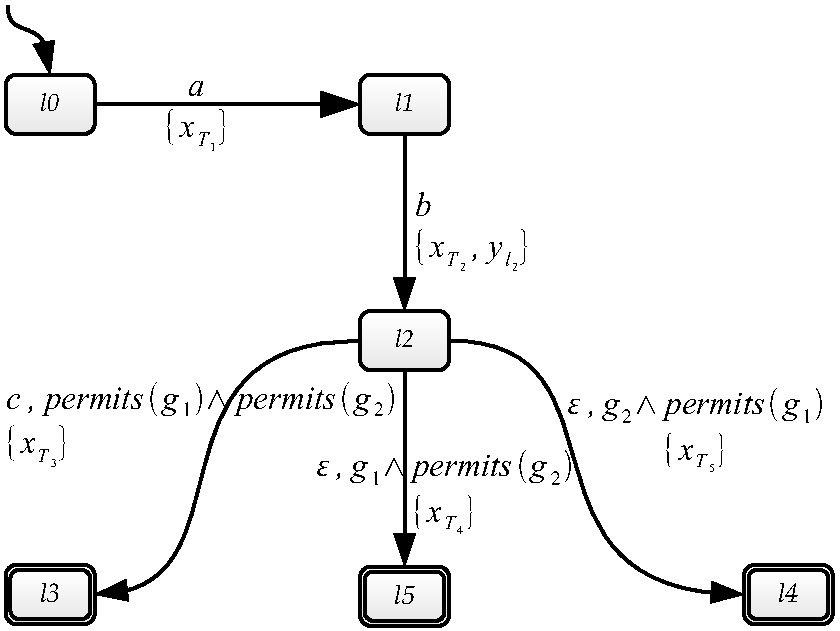
\includegraphics[width=\textwidth]{content/protocol-model/bogus-pta-constraint-fixed}
    \caption{A sample protocol timed automaton that does enforce M-Invoke semantics.}
    \label{fig:bogus-pta-constraint-fixed}
\end{figure}

The correct mapping of $\mathcal{P}$ to $A$ is given on Figure~\ref{fig:bogus-pta-constraint-fixed}, where the ``permits'' functions are just the cases that we mentioned above. For example, $\permits(g_1) = (x_{T_2} < 5) \bigvee x_{T_2} > 5) \wedge (x_{T_2} - y_{l_2} > 5)$.

% ........................................................................... %

\subsection{Protocol timed automata}

% ........................................................................... %

We named as \emph{protocol timed automata} the class of timed automata \cite{RADLD94} that we obtain by the mapping from a timed protocol that we illustrated informally in the previous section. They form a novel class of timed automata with the following characteristics:
\begin{enumerate}
  
  \item they support the empty word $\varepsilon$ as a switch label, and
  
  \item clocks are not freely added and reset on switches, they are instead split into two sets: one associates a unique clock to a unique switch while the second one associates a clock to every location that is the source of a $\varepsilon$-labeled switch, and
  
  \item the guards of $\varepsilon$-labeled switches must have at least one equality clause per possible disjunction (i.e., a clause of the form $(x = k)$ with $x$ being a clock and $k$ a rational constant or $\perp$), and
  
  \item they are deterministic, and
  
  \item the time domain is the set of positive reals $\Rpos$ augmented with the special symbol $\perp$\footnote{This symbol is used to denoted the fact that a clock is still at its initial value and has never been reset.}.
  
\end{enumerate}

The following definition gives the base of protocol timed automata. However, any automaton that satisfies this definition does not automatically enforce \MInvoke semantics. The techniques for doing that will be given later in this section.

\begin{definition}[Protocol timed automata]
Let $\T$ be the time domain defined as $\T = \Rpos \cup \{ \perp \}$.
A \emph{protocol timed automaton} $A$ is a timed automaton $A = (L, L^0, L^f, X \cup Y, E, \Sigma)$ over $\T$ such that $|L^0| = 1$ and the following conditions hold.

\begin{enumerate}

	\item For 2 switches $e = (l, g, a, r, l')$ and $e' = (l, g', a', r', l'')$ having the same source location $l$, either $a = a'$, or $g \wedge g' \models \mathtt{false}$.
	
	\item For every switch $e = (l, g, a, r, l')$, either:
	\begin{enumerate}

	 \item $l'$ is the source of a $\varepsilon$-labeled switch: $r = \{ x_e, y_{l'} \} $ with $x_e \in X$ being the clock attached to $e$ and $y_{l'} \in Y$ being the clock attached to $l'$, or
	 
	 \item $l'$ is not the source of a $\varepsilon$-labeled switch: $r = \{ x_e \} $ with  $x_e \in X$ being the clock attached to $e$.
	 
	\end{enumerate}
	It should be noted that the reset set of any switch is composed of 1 or 2 clocks.
	
	\item For every switch $e = (l, g, a, r, l')$ such that $a = \varepsilon$, $g$ is defined as a disjunction of conjunctive constraints having each at least one clock equality clause: $g = (x_1 = k_1 \wedge g_1') \vee \cdots \vee (x_n = k_n \wedge g_n')$ with $x_i$ being any clock, $k_i \in \Q \cup \{ \perp \}$ a rational constant or $\perp$, $n \in \N$ and $g_i'$ being any clocks constraint ($i \in \{1, \cdots, n \}$).

\end{enumerate}
\label{def:pta}
\end{definition}

% % ........................................................................... %
% 
% \subsection{Mapping}
% 
% % ........................................................................... %
% 
% We will use the timed protocol depicted on Figure~\ref{fig:pta-protocol} as a running example for presenting the mapping. This protocol exhibits two implicit transitions with their \MInvoke constraints.\\
% 
% We describe here how to map a timed protocol
% $$\mathcal{P} = (\mathcal{S}, s_0, \mathcal{F}, \mathtt{M}, \mathcal{X}, \mathcal{C}, \mathcal{R} \subseteq \mathcal{S}^2 \times \mathtt{M} \times \mathcal{C})$$
% to its corresponding protocol timed automaton
% $$A = (L, L^0, L^f, X \cup Y, E, \Sigma)$$
% The mapping makes use of several mapping functions, each being specialized in a portion of the mapping (e.g., one function is for states to locations, another one for transitions to edges and so on.).\\
% 
% We introduce the following mapping functions from elements of $\mathcal{P}$ to elements of $A$. Those functions are bijective.
% \begin{itemize}
%   
%   \item $\map_S: \mathcal{S} \longrightarrow L$ maps states to locations
%   
%   \item $\map_M: \mathtt{M} \longrightarrow \Sigma$ maps messages to input symbols
%   
%   \item $\map_C: \mathcal{X} \longrightarrow X$ maps transitions from $\mathcal{R}$ (each being identified by an element of $\mathcal{X}$) to clocks in $X$
%   
%   \item $\map_G: \mathcal{C} \longrightarrow \mathcal{C}(X \cup Y)$ maps temporal constraints\footnote{The notation $\mathcal{C}$ for timed protocols should not be confused with the notation $\mathcal{C}(X)$ in timed automata that denotes the set of constraints over a set of clocks $X$.} $\mathcal{C}$ of $\mathcal{P}$ to clock constraints over the set of clocks $X \cup Y$.
%   
% \end{itemize}
% 
% We now give the first step of the procedure to map $\mathcal{P}$ to $A$.
% 
% \begin{procedure}[Timed protocol mapping, step 1]
% $\mathcal{P}$ is mapped to $A$ as follows.
% \begin{enumerate}
%   
%   \item $L = \map_S(\mathcal{S})$
%   
%   \item $L^0 = \{ \map_S(s_0) \} $
%   
%   \item $L^f = \map_S(\mathcal{F})$
%   
%   \item $\Sigma = \map_M(\mathtt{M})$
%   
%   \item $X = \map_C(\mathcal{X})$
%   
%   \item For each transition $r = \mathcal{R}(s_1, s_2, m, c)$ identified by $T_{id} \in \mathcal{X}$, a switch $e = (\map_S(s_1), \map_G(c), \map_M(m), \{ \map_C(T_{id}) \}, \map_S(s_2))$ is added to $E$.
%   
% \end{enumerate}
% \label{proc:tp2pta}
% \end{procedure}
% 
% The mapping functions that we have introduced are straightforward. For example, a state $s \in \mathcal{S}$ is associated to a unique location $\map_S(s) \in L$. Similarly,
% $\map_G((T_1 < 3) || (T_2 > 4)) = (\map_C(T_1) < 3) \vee (\map_C(T_2) > 4)$. It should be noted that we allow abuse of notations such as using $\map_S$ over singletons (e.g, $\map_S(s)$) and sets (e.g., $\map_S(\mathcal{S})$).\\
% 
% At this step, the timed protocol of Figure~\ref{fig:pta-protocol} has been mapped to the timed automaton of Figure~\ref{fig:bogus-pta-constraint}. We can see how guards have been defined as well as a set of clocks. This is a relatively straightforward mapping.\\
% 
% This mapping definition is however not sufficient. Indeed, the \MInvoke constraints semantics are not enforced by the direct mapping through $\map_G$. Considering again the example on Figure~\ref{fig:bogus-pta-constraint},   the $c$-labeled switch has no guard (implicitly the guard is $g = \mathtt{true}$). If the guard of any of the $\varepsilon$-labeled switches is satisfied, then nothing actually forces it to be taken.

% ........................................................................... %

\subsection{Enforcing M-Invoke constraints in protocol timed automata}

% ........................................................................... %

We define the \MInvoke semantics so as to enforce that when the guard of a $\varepsilon$-labeled switch becomes satisfied, it is mandatorily taken. Indeed, classical timed automata augmented with $\varepsilon$-labeled switches only make the location change \emph{possible} when a guard is satisfied, not \emph{mandatory}.

\begin{definition}[\MInvoke semantics]
Let $A$ be a protocol timed automaton and $e: l \xrightarrow{\varepsilon, g} l'$ a $\varepsilon$-labeled switch of $A$. Let $v$ be the current clocks valuation such that:
\begin{enumerate}
  
  \item the current location is $l$, and
  
  \item $v \models g$
  
\end{enumerate}
In this case, the execution must immediately move to the location $l'$.
\end{definition}

Under \MInvoke semantics, the following behavior needs to be enforced (examples are taken from Figure~\ref{fig:bogus-pta-constraint}).
\begin{enumerate}
  
  \item When a $\varepsilon$-labeled switch guard becomes satisfied, all other switches must be immediately disabled so as to make it the only switch that can be taken. An example is when $g_1$ becomes satisfied in $l_2$: the two other switches must be disabled.
  
  \item When a location offering a $\varepsilon$-labeled switch is entered after the equality clause of its guard has been satisfied, the other switches must not be disabled. If $l_2$ is entered while $x_{T_2} > 5$, the other switches must not be disabled.
  
  \item When the guard of a $\varepsilon$-labeled switch cannot be satisfied when its equality clause is satisfied, the other switches must not be disabled. Let us consider $g_2$ while the current location is $l_2$. In case $(x_{T_1} = 10)$ is satisfied but $(x_{T_2} > 2)$ is not, the two other switches must not be disabled.
  
\end{enumerate}

The enforcement is done by rewriting the constraints using two functions. First, we define a function ``$\inhib$'' over a $\varepsilon$-labeled transition guard of the form $g = (x = k) \wedge g'$. The role of this function is to capture the cases where $g'$ is false, thus making the switch that has $g$ as its guard inactive. As we will see, this function plays a critical role in enforcing the \MInvoke constraints in protocol timed automata. Then, we will provide a function ``$\permits$'', also defined over a $\varepsilon$-labeled transition guard. It defines when it allows other switches from the same source location to become actionable. This function relies on the introduction of clocks that are attached to locations so as to capture the clocks valuation when locations are entered. It uses $\inhib$ that we introduce in the following definition.

\begin{definition}[$\inhib$ function]

Let a guard $g := (x = k) \wedge g'$ of a $\varepsilon$-labeled switch defined over a $\varepsilon$-labeled switch $l \rightarrow l'$ such as $x$ is a clock over $\T$, $k$ is a constant in $\Q \cup \{ \perp \}$ and $g'$ is any clocks constraint:
$ g' = 
(x_1 \;\#_1\; k_1) \wedge
 \cdots \wedge
 (x_j \;\#_j\; k_j) \wedge
 (x_{j+1} - x_{j+1}' \;\#_{j+1}\; k_{j+1}) \wedge
 \cdots \wedge
 (x_{m} - x_{m}' \;\#_{m}\; k_{m})
$
(for any $i \in \{1, \cdots, m\}$: $x_i, x_i' \in X \cup Y$, $k_i \in \Q \cup \{ \perp \}$ and $\;\#_i\;$ is any comparison operator).

We define the function $\inhib$ such that:
$
\inhib(g) =
  (x_1 - x \;\mathtt{not}(\#_1)\; k_1 - k) \vee 
  \cdots \vee 
  (x_j - x \;\mathtt{not}(\#_j)\; k_j - k) \vee
  (x_{j+1} - x_{j+1}' \;\mathtt{not}(\#_{j+1})\; k_{j+1}) \vee
  \cdots \vee 
  (x_{m} - x_{m}' \;\mathtt{not}(\#_{m})\; k_{m}) 
$

In the case where $g'$ is not defined (i.e., $g = (x = k)$), then $\inhib(g) = \mathtt{false}$.
\end{definition}

Going back to the timed automaton of Figure~\ref{fig:bogus-pta-constraint}:
$$
\left\lbrace
\begin{array}{l}
  \inhib(g_1) = \mathtt{false} \\
  \inhib(g_2) = (x_{T_2} - x_{T_1} \leq -8) \\
\end{array}
\right.
$$

Without loss of generality, we chose to reduce the $\varepsilon$-labeled switch guard $g$ to a unique conjunction in the previous definition to simplify the notations. The case where $g$ is a disjunction is easy: we consider it as multiple $\varepsilon$-labeled switches with each switch having a single conjunctive guard. We keep this assumption in the remainder.\\

With this $\inhib$ function at hand, we can now define a function called $\permits$. When given the guard of a $\varepsilon$-labeled switch, it defines when the other switches from the same source location can be enabled without contradicting M-Invoke constraints.

\begin{definition}[$\permits$ function]
  
Let a guard $g := (x = k) \wedge g'$ of a $\varepsilon$-labeled switch defined over a $\varepsilon$-labeled switch $l \rightarrow l'$ such as $x$ is a clock over $\T$, $k$ is a constant in $\Q \cup \{ \perp \}$ and $g'$ is any clocks constraint. Let $y \in Y$ the clock that is commonly reset by all the switches whose target location is $l$. We define the following clauses:
\begin{enumerate}
  
  \item $S_1 = (x < k)$
  
  \item $S_2= (x > k) \wedge (x - y > k)$
  
  \item $S_3 = (x > k) \wedge (x - y \leq k) \wedge \inhib(g)$
  
  \item $S_4 = (x = k) \wedge \inhib(g)$
  
\end{enumerate}

The function $\permits(g)$ is defined as
$$
  \permits(g) = \bigvee\limits_{i \in \{1, 2, 3, 4\}} S_i
$$
  
\end{definition}

The $\permits$ function disjunctive clauses play the following roles. $S_1$ captures the cases where the current clocks valuation $v$ ensures that $v(x)$ is still below $k$. $S_2$ captures the cases where $v$ is above $k$ and the location $l$ has been entered after $(x = k)$ was satisfied. This is checked through the clause $(x - y > k)$. $S_3$ captures the cases where $l$ was entered before $(x = k)$ was satisfied, but $g_i'$ could not be satisfied. In such cases, the switches should not be disabled for the clocks valuations such that $(x > k)$ is satisfied. Finally, $S_4$ captures the cases where $(x = k)$ is satisfied but $g_i'$ is not, hence the switches don't have to be disabled as well.\\

Again considering the timed automaton of Figure~\ref{fig:bogus-pta-constraint}:
$$
\left\lbrace
\begin{array}{lll}
  
  \permits(g_1) & =    & \underbrace{(x_{T_2} < 5)}_{S_1} \\
                & \bigvee & \underbrace{(x_{T_2} > 5) \wedge (x_{T_2} - y_{l_2} > 5)}_{S_2} \\
  
  \permits(g_2) & =    & \underbrace{(x_{T_1} < 10)}_{S_1} \\
                & \bigvee & \underbrace{(x_{T_1} > 10) \wedge (x_{T_1} - y_{l_2} > 10)}_{S_2} \\
                & \bigvee & \underbrace{(x_{T_1} > 10) \wedge (x_{T_1} - y_{l_2} \leq 10) \wedge
                            \underbrace{(x_{T_2} - x_{T_1} \leq -8)}_{\inhib(g_2)}}_{S_3} \\
                & \bigvee & \underbrace{(x_{T_1} = 10) \wedge
                            \underbrace{(x_{T_2} - x_{T_1} \leq -8)}_{\inhib(g_2)}}_{S_4} \\
  
\end{array}
\right.
$$

We can now define how the guards of the switches whose source locations offer $\varepsilon$-labeled switches need to be rewritten so as to enforce \MInvoke.

\begin{procedure}[\MInvoke enforcement]
  
Let $l$ be a location of a protocol timed automaton $A$ that offers $n > 0$ $\varepsilon$-labeled switches:
$$ \{
  e_{\varepsilon_1} = (l, g_{\varepsilon_1}, \varepsilon, r_1, l_1),
  \cdots,
  e_{\varepsilon_n} = (l, g_{\varepsilon_n}, \varepsilon, r_n, l_n)
\} $$ 

The rewriting of the guard of each switch whose source location is $l$ (including the $\varepsilon$-labeled ones) is performed as follows:
\begin{enumerate}
  
  \item for each location $l$ that offers a $\varepsilon$-labeled switch, augment the reset set of each switch whose target location is $l$ with the clock $y_l \in Y$
  
  \item compute $\{ \permits(g_{\varepsilon_1}), \cdots \permits(g_{\varepsilon_n}) \}$
  
  \item rewrite the guard $g$ of each switch $(l, g, a, r, l')$ as
  \begin{enumerate}
  	\item when $a \neq \varepsilon$
  		$$ g \bigwedge\limits_{0 \leq i \leq n} \permits(g_{\varepsilon_i})$$
  	\item when $a = \varepsilon$ and the switch guard is $g_{\varepsilon_j}$ ($j \in \{1, \cdots, m\}$)
  		$$ g \bigwedge\limits_{0 \leq i \neq j \leq n} \permits(g_{\varepsilon_i}) $$
  \end{enumerate}
  
\end{enumerate}
\label{proc:guard-rewrite}
\end{procedure}

As an example, we consider again the protocol timed automaton of Figure~\ref{fig:bogus-pta-constraint} that has been fixed to enforce M-Invoke semantics on Figure~\ref{fig:bogus-pta-constraint-fixed}.

% ........................................................................... %

\subsection{Theoretical results}

% ........................................................................... %

We now study the expressiveness of protocol timed automata, then prove that the mapping from timed protocols to timed automata is correct.

\subsubsection{Expressiveness}

\begin{theorem}
$\varepsilon$-transitions strictly increase the expressiveness of protocol timed automata.
\label{thm:mi-expressiveness}
\end{theorem}

\begin{figure}[htbp]
  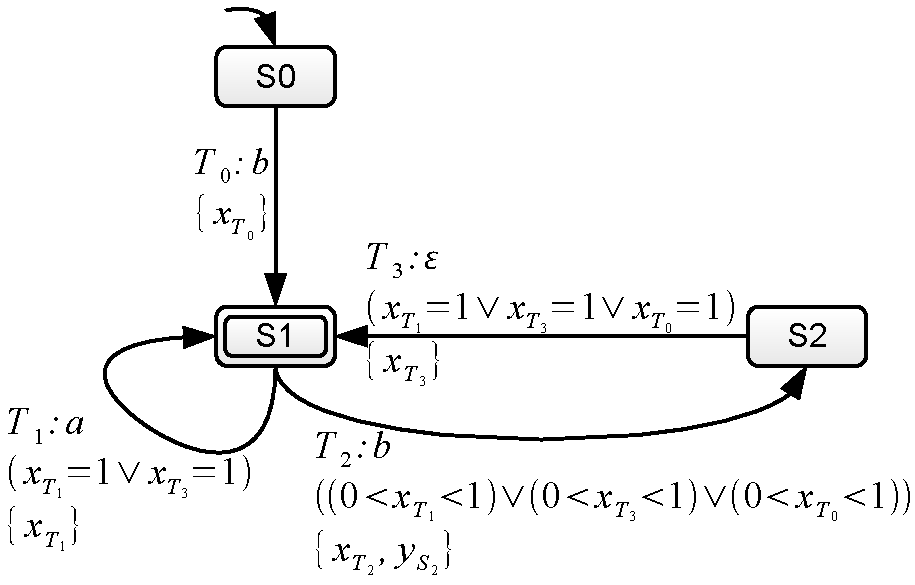
\includegraphics[width=\textwidth]{content/protocol-model/precise-time}
  \caption{A protocol timed automaton $A$ that cannot be expressed equivalently without $\varepsilon$-transitions.}
  \label{fig:precise-time}
\end{figure}

Protocol timed automata are strictly more expressive than (general) timed automata because of their $\varepsilon$-labeled switches. The proof, given on page~\pageref{proof:mi-expressiveness}, is based on the notion of \emph{precise actions} and is the same as Corollary~29 of \cite{BBVD+99}. The idea is that the protocol timed automaton of Figure~\ref{fig:precise-time} cannot be expressed equivalently by a timed automaton without $\varepsilon$-labeled switches.

\subsubsection{Correctness of the mapping}

We now give some results showing that the guards rewritings above are correct with respect to the M-Invoke constraint semantics. Indeed, the correctness of the mapping from timed protocols to protocol timed automata relies on the rewriting to correctly enforce \MInvoke constraints semantics. The following lemma shows that the function $\inhib$ works as expected, i.e., it can inhibit guards when a $\varepsilon$-labeled switch guard is totally satisfied, and allow them when it is not. The proof is given on page~\pageref{proof:inhib}.

\begin{lemma}
Let a protocol timed automaton $A$ and a location $l \in A$ such that there exists a switch $e = (l, g = (x = k) \wedge g', \varepsilon, r, l')$, with
$g' = 
(x_1 \;\#_1\; k_1) \wedge
 \cdots \wedge
 (x_j \;\#_j\; k_j) \wedge
 (x_{j+1} - x_{j+1}' \;\#_{j+1}\; k_{j+1}) \wedge
 \cdots \wedge
 (x_{m} - x_{m}' \;\#_{m}\; k_{m})$ for $m \in \N$ and $j \in \{1, \cdots, m\}$. Then:
\begin{enumerate}

  \item $(\inhib(g) = \mathtt{true}) \Longrightarrow (g' = \mathtt{false})$
  
  \item $(\inhib(g) = \mathtt{false}) \Longrightarrow (g' = \mathtt{true})$

\end{enumerate}
\label{lemma:inhib}
\end{lemma}

Given a location that has several $\varepsilon$-labeled switches, the following lemma checks that only one of them can ever become satisfied, thus disabling and forcing the transition to another location. To do that, we express the following sanity-check type of boolean implication. A proof is given on page~\pageref{proof:permits}.

\begin{lemma}
Let a protocol timed automaton $A$ and a location $l \in A$ such that it offers $n > 0$ $\varepsilon$-labeled switches. For any $i \in \{1, \cdots, n\}$, the guard $\widetilde{g_i}$ of the $i$-th $\varepsilon$-labeled switch is of the form
$$g_i \bigwedge\limits_{1 \leq i \neq j \leq n} \permits(g_j)$$

Let $i \in \{1, \cdots, n \}$ and $j \in \{1, \cdots, n\}$ such that $i \neq j$. Then:
$$
(g_j = \mathtt{true}) \Longrightarrow (\permits(g_j) = \mathtt{false}) \wedge (\permits(g_i) = \mathtt{true})
$$
\label{lemma:permits}
\end{lemma}

This implication expresses the fact that when a $\MInvoke$ guard is satisfied, then its derived $\permits$ constraint is false, and the permits clauses of every other $\MInvoke$ guards are still true. Indeed, if any of the later permits clauses was to be false, then it would mean that its guard would have already been actionable in the past, yet not taken and hence not enforced.\\

The following theorem states that the mapping of a timed protocol to a protocol timed automaton is correct with respect to \MInvoke constraints. The proof is given on page~\pageref{proof:mi-enforcement}.

\begin{theorem}
Let a protocol timed automaton $A$ obtained from a timed protocol $\mathcal{P}$ on which Procedure~\ref{proc:guard-rewrite} has been applied.
Every $\varepsilon$-labeled switch $e = (l, g = (x = k) \wedge g', \varepsilon, r, l')$ of $A$ is taken as soon as its guard $g$ is satisfied.
\label{thm:mi-enforcement}
\end{theorem}

Finally, the following lemma states that protocol timed automata are deterministic. The proof is given on page~\pageref{lemma:pta-determinism}.

\begin{lemma}
Protocol timed automata are deterministic: given a protocol timed automaton $A$ and a timed word $w \in \mathcal{L}(A)$, $w$ has exactly one run over $A$.
\label{lemma:pta-determinism}
\end{lemma}

% ........................................................................... %

\section{Discussion}

% ........................................................................... %

The following discussion aims at first positioning protocol timed automata with respect to event-clock automata as defined in \cite{RALF94}. We then discuss two potential limitations in our model. The first is the absence of support for absolute time constants (e.g., supporting constraints of the form $(x < \mbox{\texttt{2008-05-10:20:00:00}})$). The second one is the assumption that we do not take into account network transport delays and losses. 

% ........................................................................... %

\subsection{Relationship to event-clock automata}

% ........................................................................... %

The class of protocol timed automata can be seen as an extension of event-recording automata \cite{RALF94}. In fact, their design has been made with them in mind. Yet, any protocol timed automaton is not necessarily a event-recording automaton. One straightforward similarity between the two classes is the time domain $\T = \Rpos \cup \{ \perp \}$ and that clocks are assigned and reset in a restricted fashion. There are however several differences:
\begin{itemize}
  
  \item protocol timed automata support $\varepsilon$-labeled switches with clock resets, and
  
  \item some particular switches may reset two clocks (i.e., the ones whose target location offers a $\varepsilon$-labeled switch), and
  
  \item one subset of the clocks assigns them to switches (i.e., $X$), not input symbols, while the complement subset assigns them to locations ($Y$).
  
\end{itemize}

However as we will see in the next chapters, protocol timed automata are fully deterministic, and they have the property that the value of clocks only depends of the input words, despite $\varepsilon$-labeled switches (at first sight, one would think that they necessarily introduce indeterminism).\\

The class of event-recording automata is however a subset of protocol timed automata. Indeed, let us consider an event-recording automaton: it can be translated directly to a protocol timed automaton $A$ as:
\begin{enumerate}
  
  \item there is no $\varepsilon$-labeled switch, and
  
  \item for every input symbol $a$ and any guard clause of the form $(x_a \;\#\; k)$ ($\#$ is any operator and $k$ a constant), it can be rewritten as $(x_{e1} \;\#\; k) \vee \cdots \vee (x_{en} \;\#\; k)$ where $\{ x_{e1}, \cdots, x_{en} \}$ is the set of switches in $A$ where $a$ is the input symbol.
  
\end{enumerate}

\begin{figure}[htbp]
	\centering
  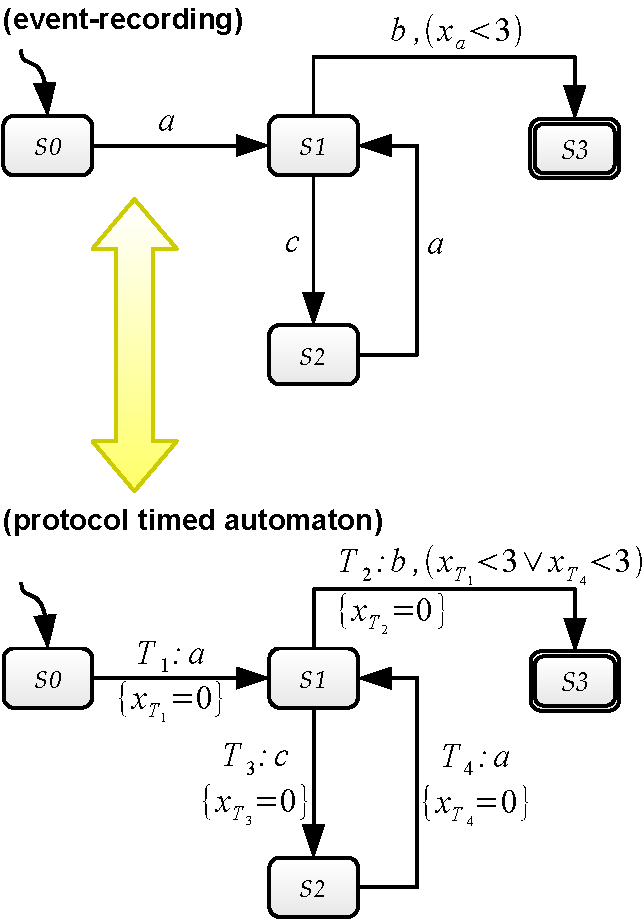
\includegraphics[width=0.7\textwidth]{content/protocol-model/era}
  \caption{A sample event-recording automaton viewed as a protocol timed automaton.}
  \label{fig:era}
\end{figure}

We give an example on Figure~\ref{fig:era} of a event-recording timed automaton encoded as a protocol timed automaton.

% ........................................................................... %

\subsection{Constraints with absolute dates}

% ........................................................................... %

Timed protocol constraints are always expressed relatively to a transition of a given protocol being fired (e.g., $\CInvoke(T_1 < 3h)$). Absolute dates cannot be used in constraints (e.g., $\CInvoke(T_1 < \mbox{'2007-04-19 14:49:00'})$ or $\CInvoke(\mbox{current\_time} < \mbox{'2007-04-19 14:49:00'})$). Such types of constraints can be found in some specifications such as BPEL \cite{WSBPEL2} where both types of \emph{relative} and \emph{absolute} time expressions can be used.\\

Let us briefly investigate the impact of introducing absolute dates into the model by looking at the involved mechanisms at the timed automata level. Allowing a constraint to compare a clock $x$ to a constant $date$ (e.g., $x < \mbox{'2007-04-19 14:49:00'}$) which represents an absolute date requires the following assumptions.
\begin{enumerate}
    \item $x$ is set to a constant $now$ which represents the current date when the automaton execution starts, and
    \item $x$ is always compared to absolute dates, and
    \item $x$ is never reset in the considered automaton.
\end{enumerate}

We claim that making such an extension renders the timed language emptiness checking problem undecidable. The proof can be done by observing that $now$ is actually a variable. In timed automata, the clocks are set to a constant value (usually $0$) when the execution starts. Here, we would have some special clocks that would be initially set to a value which depends on the current time. Hence, the result of checking for the emptiness of such an extended timed automaton would only hold considering the time at which the checking has been performed (i.e., the results holds at time $t$ but may not hold anymore at time $t + \delta$ with any $\delta \in \Rpos$).\\

This limitation of timed protocols in terms of expressiveness is not a penalty as such constructs are of limited use in practice. In the case of BPEL, timers are mainly used for generating timeout exceptions in asynchronous operations (e.g., the \emph{pick} complex activity). They can be also used for a \emph{wait} activity (e.g., put the process in sleep). In our experience, we have never found a need for expressing absolute dates in BPEL processes. Also, \emph{JBoss JBPM} (see \url{http://www.jboss.com/products/jbpm}), a widely used business process management system, offers a workflow language called \emph{jPDL} where time-related constructs are always expressed in a relative manner (i.e., \emph{jPDL} does not allow specifying absolute dates for timers).

% ........................................................................... %

\subsection{Message transport communications}

% ........................................................................... %

Our model is based on the assumption that there are no message transmission delays and losses. This is of course not the case in reality as web services messages are mostly transported over unreliable networks that can have substantial load variations, leading to greatly varying network latencies and even errors. The class of \emph{Robust Timed Automata} \cite{RAPM04} is a possible exploration path for solving those issues. Briefly, a robust timed automaton recognizes timed words with some fuzziness in the event dates as no real world system can be expected to be as precise as timed automata expectations. The classical decidability problems (reachability / emptiness, inclusion) remain unchanged for this class. However, the expressiveness of such automata cannot be compared to the one of timed automata \cite{RAPM04}. That is why we guess that using them as a formal framework for timed protocols probably requires substantial investigations from a theoretical point of view.

% % ........................................................................... %
% 
% \subsection{Inverse mapping: from protocol timed automata back to timed protocols}
% 
% % ........................................................................... %
% 
% Given a protocol timed automaton
% $$A = (L, L^0, L^f, X \cup Y, E, \Sigma)$$
% its corresponding timed protocol
% $$\mathcal{P} = (\mathcal{S}, s_0, \mathcal{F}, \mathtt{M}, \mathcal{X}, \mathcal{C}, \mathcal{R} \subseteq \mathcal{S}^2 \times \mathtt{M} \times \mathcal{C})$$
% can easily be obtained as follows. The construction is relatively easy given the mapping described in Procedure~\ref{proc:tp2pta}, hence we will keep the discussion rather informal.\\
% 
% The mapping functions used in Procedure~\ref{proc:tp2pta} support direct inverse functions. For example the mapping from locations in $A$ to states in $\mathcal{P}$ is given by
% $$ \map_S^{-1}: L \longrightarrow \mathcal{S} $$
% that associates to each location a location in $\mathcal{S}$.\\
% 
% The inverse mapping requires two preliminary steps:
% \begin{enumerate}
%   
%   \item remove the $\permits$ clauses from the guards in $A$, then
%   
%   \item remove the set of clocks $Y$ in $A$ (these clocks are only used in $\permits$ clauses).
%   
% \end{enumerate}
% When this is done, the inverse mapping functions can be applied to infer a timed protocol.\\
% 
% Consider the protocol timed automaton of Figure~\ref{fig:bogus-pta-constraint-fixed}. The first two steps presented below yield the timed automaton of Figure~\ref{fig:bogus-pta-constraint}. Applying inverse functions gives back the timed protocol first introduced on Figure~\ref{fig:pta-protocol}.

% ........................................................................... %